\documentclass{article}
\pdfpagewidth=8.5in
\pdfpageheight=11in
\usepackage{ijcai27}
% The kit says 'Use the postscript times font!'. Under XeTeX, \usepackage{times} silently falls
% back to Latin Modern (TU/ptm/m/n undefined), so the typeface is set explicitly instead.
% TeX Gyre Termes is a Times clone and ships with the engine's bundle, so the build is portable.
\usepackage{fontspec}
\setmainfont{texgyretermes}[Extension=.otf, UprightFont=*-regular, BoldFont=*-bold,
  ItalicFont=*-italic, BoldItalicFont=*-bolditalic]
\setmonofont{texgyrecursor}[Extension=.otf, UprightFont=*-regular, BoldFont=*-bold,
  ItalicFont=*-italic, BoldItalicFont=*-bolditalic, Scale=0.9]
\usepackage{unicode-math}
\setmathfont{texgyretermes-math.otf}
\usepackage{url}
\usepackage[hidelinks]{hyperref}
\usepackage[utf8]{inputenc}
\usepackage[small]{caption}
\usepackage{graphicx}
\usepackage{amsmath}
\usepackage[switch]{lineno}
\usepackage{booktabs}
\providecommand{\tightlist}{\setlength{\itemsep}{0pt}\setlength{\parskip}{0pt}}
\urlstyle{same}

\begin{document}
\linenumbers

\title{Allocation Was Never the Bottleneck: What Actually Moves a Protein-Fitness Ranker}

% Anonymous submission: no author block.
\author{}
\maketitle

\begin{abstract}
Protein engineering screens rank candidate mutations, but the field optimises the fusion of sequence and
structure models. We test that premise on the ProteinGym substitution benchmark, 217 assays and 651
assay-by-split units, and find that every one of seven adaptive weighting mechanisms we measured ties a
single constant tuned on held-out assays. A per-assay oracle bounds the entire headroom any weighting
rule could capture at +0.0027, against +0.0077 for replacing a single expert. A second benchmark --
ProteinGym's indel assays, a different mutation type and a different expert pool -- shows the bound has
two parts: its oracle gap is three times larger there, yet weights fitted on half an assay's variants lose
to a fixed blend on the other half, and assay size decides which part binds. We then show where the
headroom is: an encoder over reference-minus-mutant representations in a local neighbourhood, distilled
from the strongest experts, with a category-specific low-rank residual and eight-seed averaging, fused
as four fixed weights reaches 0.694 on the official metric against 0.657 for the published leader. The
useful result for the domain is the shape of the ranking: the top 5\% recovers 24.7\% of the true top
5\%, a 4.96x lift, but 7.7x on stability assays against 3.4x on activity. We release per-mutant
predictions for all 696,311 mutants.
\end{abstract}
\section{Introduction}\label{introduction}

A protein engineering campaign begins with a library of candidate mutations and a budget covering tens
of assays, perhaps hundreds. Everything upstream of the bench is a ranking problem: which candidates are
worth synthesising. The models that answer it have improved substantially --- sequence language models
\cite{esm2}, structure-informed kernels \cite{kermut}, supervised models trained on deep mutational
scanning data \cite{proteinnpt} --- and the practice is to combine several, because they fail on different
assays \cite{proteingym}.

The combination is almost always \textbf{conditional}: a gate reads assay-level context and emits weights, a
mixture layer routes by protein family \cite{jacobs1991,shazeer2017}, an uncertainty term reweights per
variant \cite{deepsong}. The premise is that different assays need different mixtures, and that learning
the mapping from context to weights is worth its parameters. It has produced a decade of architectures.

This paper tests it, and the answer reorganises the problem.

\textbf{First, the allocation headroom is small enough to bound.} We evaluate six label-free conditioning
mechanisms --- parametric and nonparametric, per-assay, per-category and per-variant, supervised and not ---
against a single constant tuned on held-out assays. One clears it, by +0.00025 with a confidence interval
straddling zero; four land within 0.0006 below. The sharper statement is an oracle: a rule that sees the
held-out assay's own labels can gain \textbf{+0.0027} over the fixed blend, and that is the ceiling for any
weighting of this pool. Replacing one expert is worth \textbf{+0.0077} in the same protocol. \textbf{The entire
allocation headroom is a quarter of the expert headroom.}

\textbf{Second, the expert headroom is in how a mutation is represented.} A substitution is a difference
between two sequences, and the useful signal is the difference --- not the mutant residue in isolation, not
the site in isolation. We build an encoder over reference-minus-mutant features in a ±4-residue
neighbourhood, distilled from the agreement of the two strongest experts, with a functional-category
low-rank residual and predictions averaged over eight seeds. Fused with three published experts at four
fixed weights, it reaches \textbf{0.694} on the official ProteinGym metric against \textbf{0.657} for Kermut, the
leaderboard leader. We validate the measurement before reporting it: recomputing Kermut through our
pipeline reproduces the published per-assay table on all 217 assays with mean absolute difference 0.0.

\textbf{Third, an aggregate score is not a deployment specification, and we report the one that is.} The same
model that reaches 0.694 overall scores 0.851 on stability assays and 0.642 on activity assays, and the
ordering it produces is uneven in the same way: the top 5\% of the ranking recovers 24.7\% of the true top
5\%, a \textbf{4.96x} lift over random, which rises to 7.7x on stability and falls to 3.4x on activity. The
advantage also has a size regime --- largest on small assays, and at parity with the previous fusion
(+0.00003) on the largest quartile of mutant counts. Those two numbers are what let a laboratory decide
how much of the ordering to trust for its own property and its own assay size.

The second claim is what changes how the field builds these models; the third is what a user can act on
today; the first is what makes both measurable rather than asserted.

\subsection*{Contributions}\label{contributions}

\begin{enumerate}
\def\labelenumi{\arabic{enumi}.}
\tightlist
\item
  \textbf{A falsification of adaptive weighting for this problem, replicated on a second benchmark.}
  Seven mechanisms under one protocol, all at or below a tuned constant, plus an oracle bounding the
  total allocatable gain at +0.0027. On ProteinGym's indel assays the same bound is measured and shown to
  have a second part: how much of it the assay can estimate. We argue both the oracle and the tuned
  constant belong in the baseline table.
\item
  \textbf{An expert built from differential representations}, with the ablation that shows where the signal
  is: the wild-type-minus-mutant difference and the local neighbourhood carry +0.116, while stacking
  more layers alone is negative.
\item
  \textbf{A utility characterisation that makes the ranking usable} --- top-of-list recall by functional
  category, and the assay-size regime over which the advantage holds. It converts one aggregate number
  into the two facts a campaign needs: how much of the top of the list to trust, and for which property.
\item
  \textbf{A reproducible artifact}: per-mutant predictions for all 696,311 mutants and the code that
  regenerates every number in two commands from two public repositories, supplied with this submission
  as anonymised supplementary material and released publicly on publication.
\end{enumerate}

\section{Related work}\label{related-work}

\textbf{Protein fitness prediction.} Three lines converge here. Zero-shot predictors score variants from a
sequence model's likelihood or from multiple-sequence-alignment statistics, without touching assay labels
\cite{esm1v,tranception,msatransformer}. Supervised approaches train on deep mutational scanning data
\cite{fowler2014,yang2019}, either per assay or across a panel; the leaderboard leader is a composite
kernel regression of this kind. The fusion line, which this paper belongs to, combines predictors that
fail differently, and the combination is usually weighted per assay. Benchmarks for this comparison are
themselves a design choice \cite{flip}, and §5.1 therefore verifies the one we use end to end before
reporting any comparison on it.

\textbf{Adaptive weighting and gating.} Mixture-of-experts layers and context-conditioned gates are standard
across machine learning, usually justified by heterogeneity of the input distribution. Our negative
result does not contradict that literature; it identifies a regime where the justification fails --- the
mixture components are correlated at 0.78 to 0.96 within a unit, and the conditioning variable is not the
one the optimal weights depend on. Reported gains for gating in such regimes should be read against a
tuned constant rather than a fixed prior, and against an oracle.

\textbf{Evaluation practice in AI for science.} Aggregate correlation is the standard reporting unit and a poor
guide to deployment: it is insensitive to where in the ranking errors fall, and it averages over
subpopulations a practitioner treats separately. Our top-of-list analysis by functional category is a
step toward reporting what a downstream experiment would experience.


\begin{figure}[t]
\centering
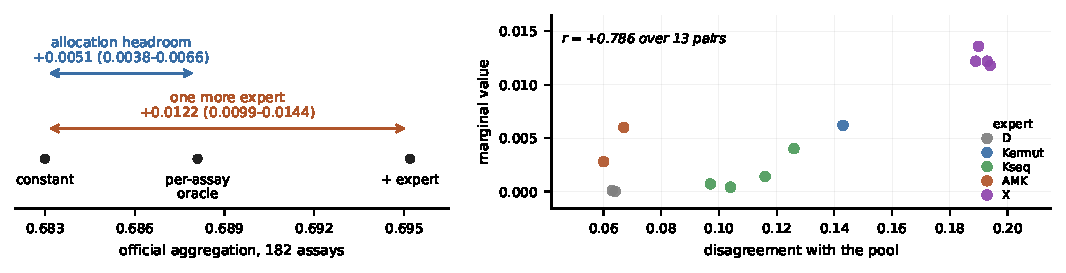
\includegraphics[width=0.86\columnwidth]{../figures/fig1_allocation_vs_expert_ijcai.pdf}
\caption{Allocation headroom against expert headroom, same protocol. The shaded band spans what any
weighting rule could gain over a tuned constant (a per-assay oracle, +0.0027); the lower arrow spans
what replacing one expert gained (+0.0077). Every adaptive mechanism we measured lands inside or below
the band.}
\label{fig:allocation}
\end{figure}

\section{Allocation has no headroom}\label{allocation-has-no-headroom}

This section establishes that the mixture has nowhere to go. We first evaluate six label-free conditioning mechanisms against a tuned constant, then bound what \emph{any} weighting rule could extract from this expert pool, then show that the bound is reproducible rather than an artefact of fitting
noise.

\subsection{Protocol and reproducibility}\label{protocol-and-reproducibility}

\textbf{Benchmark and aggregation.} ProteinGym's supervised substitution benchmark: 217 assays over 186
UniProt identifiers, each with the three official splits, giving 651 assay-by-split units. We use the
benchmark's own aggregation chain unmodified --- per-unit Spearman, averaged over splits, grouped by
UniProt identifier and coarse functional category, then averaged over the five categories --- and run its
published evaluation script on a score file we supply rather than reimplementing the metric. The grouping
step is the one most often skipped: several assays share a protein, and averaging before the category step
moves the result by about 0.005.

\textbf{Models.} Four experts: two frozen published predictions (Kermut, an assay-adaptive mixed structure
kernel), an additive structure kernel that receives weight 0.00 and does not affect scoring, and the
encoder of §4, refitted per assay and per split. Feature construction, the distillation loss, the
category residual and the seed averaging are specified in §4; α and the residual rank were re-selected by
inner selection on training assays only.

\textbf{Fusion.} Four weights per fold by step-0.1 simplex search on the training assays, applied to the
held-out ones --- the same procedure the tuned-constant baseline uses, so the comparison is equal-compute.

\textbf{Baselines.} Five, in increasing strength: a fixed 50/50 blend of the two strongest experts; a fixed
D+Kermut blend; the tuned constant of §3; a nested constant with per-fold weights; and Kermut alone, which
is also the published leaderboard leader.

\textbf{Statistics.} Seed intervals from eight independent full-pipeline runs; assay intervals from a two-level
bootstrap resampling assays within category and seeds together, 4,000 replicates. Comparisons between two
configurations on the same assays use paired differences, because assay-to-assay variance is an order of
magnitude larger than the effect.

\textbf{Compute and reproduction.} One H200 GPU per encoder run, a few hours for a full panel with eight seeds;
the structural experts are frozen and cost nothing at scoring time. Two commands from two public
repositories regenerate every number here, and the control row of §5.1 is produced by the same command as
the headline, so a reader can check our aggregation before trusting any comparison built on it.

\subsection{Seven mechanisms, one protocol}\label{seven-mechanisms-one-protocol}

We evaluate six label-free conditioning mechanisms plus the tuned constant they all must beat, on
ProteinGym \cite{proteingym}: 217 substitution assays, 651 assay-by-split units, official
category-balanced aggregation. Every mechanism is label-free with respect to the assay being scored ---
its weights for assay \emph{a} come from other assays or from no labels at all. A model is refitted per assay
on four of five published folds and predicts the fifth; our folds are bit-identical to the released
files, verified on all three schemes for a 9,576-variant assay.

\begin{table*}[t]
\centering
\small
\begin{tabular}{lrrr}
\hline
mechanism & official & $\Delta$ vs constant & 95\% CI \\
\hline
tuned constant (0.05, 0.45, 0.50) & \textbf{0.687637} & --- & --- \\
MLP gate over 17 context statistics & 0.687888 & \textbf{+0.000251} & [-0.001924, +0.002545] \\
per-variant uncertainty weighting & 0.687106 & -0.000531 & [-0.001181, +0.000021] \\
k-NN over assay context & 0.687170 & -0.000467 & [-0.001329, +0.000259] \\
per-category constants & 0.687220 & -0.000417 & [-0.000784, -0.000084] \\
ridge context → weights & 0.685109 & -0.002528 & [-0.007833, +0.000676] \\
per-variant consensus (median) & 0.670492 & -0.017146 & [-0.026771, -0.011115] \\
\hline
\end{tabular}
\end{table*}

One mechanism clears the constant, by +0.00025, with a confidence interval straddling zero; four more
land within 0.0006 below it, the same magnitude on the other side. The two that fail badly do so
instructively --- a context regressed onto weights scores below the constant, so the regression is actively
harmful, and a per-variant median discards the magnitude that separates a strong predictor from a weak
one. \textbf{No mechanism is separated from a tuned constant by more than the seed-to-seed spread of the models
themselves.}

\subsection{The bound is small}\label{the-bound-is-small}

The oracle over the same expert pool reaches \textbf{0.693544}, against \textbf{0.690808} for the fixed blend --- a
headroom of \textbf{+0.0027}. That is the entire amount any weighting rule, supervised or not, per-assay or
not, could ever extract from this pool. For comparison, the same protocol attributes \textbf{+0.0077} to
replacing a single expert.

\textbf{The allocation headroom is a quarter of the expert headroom.} That is the paper's central magnitude
comparison. The gate itself does what its designers would want --- its per-assay weights reproduce across
independent seeds at r = 0.92--0.97, and shuffling them within category costs 0.0017 --- which locates the
problem in the objective rather than in the optimisation: the pool does not contain enough disagreement
for the choice to matter. The tuned optimum places
weight 0.05 on the additive-structure expert, and deleting that expert entirely costs nothing measurable.

\subsection{The headroom is real, and it is not noise}\label{the-headroom-is-real-and-it-is-not-noise}

A small oracle gain invites the objection that the oracle is fitting its own noise. Variants of each
assay are split into disjoint halves A and B; weights selected on A and evaluated on B transfer a gain of
\textbf{+0.0041}, which is \textbf{49\%} of the +0.0083 obtainable when selection and evaluation share variants. Half
the oracle gain survives contact with unseen variants, so the per-assay optimum is a stable property of
the assay rather than an artefact of selection.

That half-surviving gain is still three times what any mechanism captures, which sharpens the diagnosis:
the headroom exists, it is reproducible, and it is not a function of the context statistics anyone
computes. A ridge \cite{rasmussen2006} from the same 17 statistics to the oracle weights, with leave-one-out
protection, reaches 0.6860 --- below the constant, meaning the fitted direction is actively wrong.

\subsection{A second benchmark: the bound has two parts}\label{a-second-benchmark-the-bound-has-two-parts}

We repeat both measurements on ProteinGym's \textbf{indel} benchmark --- 66 assays, 287,207 variants, a
different mutation type, and a different expert pool: three published supervised indel models whose
out-of-fold predictions ship with the benchmark, so this half involves no training and the comparison is
exact.

\begin{table*}[t]
\centering
\small
\begin{tabular}{lrr}
\hline
 & substitution benchmark & indel benchmark \\
\hline
per-assay oracle minus tuned constant & +0.0027 & \textbf{+0.0084} \\
share of that gap surviving a held-out-variant split & 49\% & \textbf{-19\%} \\
median variants per assay & thousands & \textbf{154} \\
\hline
\end{tabular}
\end{table*}

The oracle gap is three times larger on indels, which on its own would say allocation headroom is
substantial here. The split test says otherwise: weights selected on half an assay's variants \textbf{lose} to
the constant by 0.0024 on the other half --- negative in all ten random splits we drew (±0.0020) --- where the
same procedure on substitutions transfers 49\% of the in-place gain. The difference is assay size. Across indel assay-size quartiles the transfer is −0.0053,
−0.0023, −0.0002 and \textbf{+0.0044}; only the largest, at a median of 490 variants, recovers part of what an
oracle fitted in place suggests.

\textbf{The representation transfers, and it carries its own weight.} We build our differential encoder for
indels --- the same wild-type/mutant difference and ±4 neighbourhood, with the edit site located by longest
common prefix and suffix --- and train it under ProteinGym's released per-variant fold assignment, so our
out-of-fold predictions sit on the same split as the published models. The 226k-variant AAV library is
excluded for runtime, leaving 65 assays.

On measured fitness alone, with no distillation, it scores \textbf{0.8401} against 0.8231 for the best published
model and lifts the three-expert blend from 0.8438 to \textbf{0.8546}. Distilling from the three published models
then adds a further 0.046, reaching \textbf{0.8858} and a four-expert blend of \textbf{0.8934}. The weighting headroom
is unchanged throughout --- between +0.006 and +0.009 across every pool we trained, against +0.0084 for the
three published models alone. A much stronger pool moves the level, not the allocation bound.

Per-assay weighting is therefore limited twice: by how much the pool disagrees, which the oracle measures,
and by whether the assay carries enough variants to estimate the weights at all. Substitutions have a
small first bound and a partly estimable one; indels have a larger first bound that is almost entirely
estimation noise. \textbf{Assay size, not only pool diversity, decides whether adapting weights is worth
attempting} --- a rule that a practitioner can apply before fitting anything.

\subsection{What this means for the field}\label{what-this-means-for-the-field}

\textbf{Report against tuned constants, not fixed blends.} A gate beating a fixed 50/50 blend by +0.0047 is
commonly reported as evidence that conditioning works; against a constant tuned on held-out assays the
same gate is +0.0002, a statistical tie. The gain attributed to conditioning is mostly the gain from
\emph{tuning at all}.

\textbf{A per-assay oracle should be a reported baseline.} It costs nothing to compute and converts ``our gate
improves over the previous gate'' into ``our gate captures \emph{x} percent of the available headroom'', which is
the only number telling a reader whether the mechanism is worth its complexity. Here \emph{x} is four percent.

\textbf{When the oracle is small, the pool is the problem.} If no weighting of these experts can gain more
than +0.0027, the next +0.01 has to come from an expert that disagrees usefully. §4 builds one.

The claim is bounded by the pool: the oracle is a function of how much the experts disagree, so a pool
built to disagree might make gating worthwhile again --- a different paper, and one that would have to
report the oracle too.

\section{The expert}\label{the-expert}

If allocation is exhausted, the headroom has to be in the experts. This section builds one from a different view of the same information, and then asks which of its design choices actually carry the
gain --- including one that looks like capacity and turns out to be structure.

\subsection{What a mutation is, as a signal}\label{what-a-mutation-is-as-a-signal}

A substitution is a difference. We extract per-residue representations from three ESM-2 650M layers
\cite{esm2} (20, 30, 33) on both the wild-type and the mutated sequence, keep \texttt{mut}, \texttt{wt} and \texttt{mut\ −\ wt},
and pool a ±4-residue window by mean at layers 30 and 33. The union is 12,800 dimensions per variant. The
ladder under the per-assay protocol says where the signal comes from:

\begin{table*}[t]
\centering
\small
\begin{tabular}{lr}
\hline
representation & score \\
\hline
site vector only (layer 33) & 0.467 \\
+ multiple layers & 0.464 \\
+ ±4 neighbourhood & 0.480 \\
\textbf{+ wild-type layers and difference terms} & \textbf{0.596} \\
\hline
\end{tabular}
\end{table*}

Stacking layers alone is negative; the gain is in the difference and the wild-type context, worth +0.116,
an order of magnitude more than either other step.

\subsection{Distillation, and a residual per functional category}\label{distillation-and-a-residual-per-functional-category}

A 12,800-dimensional head trained on a few thousand variants per assay overfits before it learns. We
regularise it with the two strongest experts: their per-assay z-scores give a teacher
\texttt{t\ =\ 0.4·Kermut\_z\ +\ 0.5·AMK\_z}, and the loss is \texttt{(1\ −\ α)·MSE(student,\ target)\ +\ α·MSE(student,\ teacher)}
with α = 0.9. Re-selecting α inside each of the five folds, using only training assays, picks 0.9 in all
five. Distillation is worth +0.114 on the union representation --- the largest single step in the encoder's
development, larger than the feature union itself.

Assays fall into five categories that behave differently, so we add a low-rank correction to the head:
\texttt{y\ =\ MLP(x)\ +\ U\_c\ V\_cᵀ\ x}, with \texttt{U\_c} zero-initialised and rank 8, \texttt{c} the assay's category. The branch is
worth \textbf{+0.024} standalone and \textbf{+0.0014} in the fusion --- the gap is the decorrelation argument in
miniature, since a residual that makes an expert better can make it less useful to a pool already holding
what it learned.

\textbf{The control that decides the interpretation.} A shared branch with the same rank has one fifth of the
parameters and is indistinguishable from no branch (−0.0008, 2/4 seeds); the per-category branch beats it
by \textbf{+0.0214} standalone with every seed positive, on a matched per-branch comparison. \textbf{The gain needs
the category structure, not the parameters.} Rank 4 and rank 8 differ by 0.0002, so the branch is
saturated far below what memorising a category would require.

\subsection{Variance, and four fixed weights}\label{variance-and-four-fixed-weights}

Eight independent runs of the same architecture differ by about 0.004 in the official metric. We average
the predictions per variant rather than the scores: +0.023 standalone, +0.0022 in the fusion, the
asymmetry being that the fusion already averages four experts.

The fusion is four numbers, \texttt{0.00·D\ +\ 0.40·Kermut\ +\ 0.40·AMK\ +\ 0.20·X}, selected on the training assays
of each fold and applied to the held-out ones --- exactly the protocol the tuned constant uses. The search
drives the additive-structure weight to 0.00 in 14 of 15 seed-by-fold cells and sets the new expert to
0.20 in all 15. Under the official metric:

\begin{table*}[t]
\centering
\small
\begin{tabular}{lr}
\hline
configuration & official \\
\hline
previous four-expert fusion & 0.685538 \\
+ distilled encoder, category residual & 0.691130 \\
\textbf{+ eight-seed averaging} & \textbf{0.693311} \\
\hline
\end{tabular}
\end{table*}

against \textbf{0.657028} for Kermut \cite{kermut} --- +0.0085 over the previous fusion, +0.037 over the leader.

\subsection{What the ablation rules out}\label{what-the-ablation-rules-out}

\textbf{Co-distillation from the fusion itself} lifts the expert by +0.0136 (8/8 seeds) and leaves the fusion
at −0.0002: teaching an expert to imitate the pool removes the residual disagreement that gave it value.
\textbf{A residual expert} trained on the fusion's own error receives weight exactly zero in every fold --- the
residual of a fitted ensemble is what these features cannot explain. \textbf{A larger backbone} (ESM-C 300M)
is decorrelated but too weak: +0.0007 as a fourth expert with an interval straddling zero, and −0.011
concatenated. Representation diversity without competence buys nothing.

The constructive reading: an expert earns its place through disagreement in the residual, and the way to
get that disagreement is a different \emph{view} of the same information --- reference versus mutant, local
versus global --- not a different optimiser, loss, or a bigger model.


\begin{figure}[t]
\centering
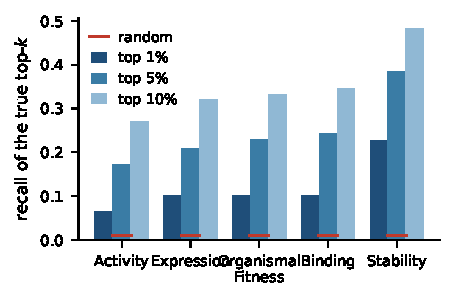
\includegraphics[width=0.86\columnwidth]{../figures/fig2_topk_by_category_ijcai.pdf}
\caption{Top-of-list utility by functional category: recall of the true top-$k$ variants when the top
$k$ of our ranking is taken, for $k \in \{1\%, 5\%, 10\%\}$, with the random-ordering expectation
marked. Stability is consistently strongest and activity weakest, a spread the aggregate Spearman does
not reveal.}
\label{fig:topk}
\end{figure}

\section{What the ranker is worth}\label{what-the-ranker-is-worth}

The preceding sections argue about where gain comes from. This one asks what the resulting ranker is worth: first on the benchmark's own terms, then on the terms a laboratory actually uses, and finally where it does
not help --- which is the part most papers leave out.

\subsection{Measuring it the way the leaderboard measures it}\label{measuring-it-the-way-the-leaderboard-measures-it}

We run the official \path{performance_DMS_supervised_benchmarks.py} unmodified on a score file of our
per-assay, per-scheme correlations, and as a control we run the same correlations recomputed from
Kermut's predictions. The control reproduces the published per-assay table on \textbf{217 of 217 assays} with
mean absolute difference \textbf{0.0}, the residual being the published table's three-decimal rounding, and
our folds are bit-identical to the released distribution.

\begin{table*}[t]
\centering
\small
\begin{tabular}{lrrrr}
\hline
model & official & random & modulo & contiguous \\
\hline
Kermut (published rank 1) & 0.657 & 0.745 & 0.633 & 0.593 \\
our fusion, single model & \textbf{0.691} & 0.782 & 0.671 & 0.624 \\
our fusion, seed-averaged & \textbf{0.694} & 0.784 & 0.674 & 0.625 \\
\hline
\end{tabular}
\end{table*}

Kermut is one of the four experts, so this is a fusion result and we report it as such: +0.037 is what
adding two complementary experts to the strongest published single model is worth. The equal-compute
comparison is the single-model rung above --- one trained expert instead of eight averaged ones --- which
still leads Kermut by 0.034.

\subsection{The aggregate hides the category, and the top of the list}\label{the-aggregate-hides-the-category-and-the-top-of-the-list}

Per functional category:

\begin{table*}[t]
\centering
\small
\begin{tabular}{lrrr}
\hline
category & ours & Kermut & delta \\
\hline
Stability & \textbf{0.851} & 0.817 & +0.034 \\
Expression & 0.693 & 0.670 & +0.023 \\
Binding & 0.653 & 0.611 & +0.042 \\
Activity & \textbf{0.642} & 0.605 & +0.037 \\
OrganismalFitness & 0.632 & 0.582 & +0.050 \\
\hline
\end{tabular}
\end{table*}

Every category improves, and the spread is the part that matters downstream: 0.851 against 0.642 is a
0.21 gap, so a laboratory working on an activity assay is operating at the bottom of the range we report.

Spearman is a whole-list statistic. A campaign has a library and can assay tens of candidates, so the
question is whether the top of our ranking contains the top of the true ranking. For each assay and split
we take the top \emph{k} ∈ \{1\%, 5\%, 10\%\} and measure how many land in the true top \emph{k}, aggregating the
official way:

\begin{table*}[t]
\centering
\small
\begin{tabular}{lrrr}
\hline
top of the list & recall of the true top & random & lift \\
\hline
1\% & \textbf{0.119} & 0.010 & \textbf{11.8x} \\
5\% & \textbf{0.247} & 0.050 & \textbf{4.96x} \\
10\% & \textbf{0.350} & 0.100 & \textbf{3.50x} \\
\hline
\end{tabular}
\end{table*}

Ordering the top 5\% recovers about a quarter of the true top 5\%, roughly five times random. It is also
category-dependent, in the direction the category table above predicts: 7.7x on Stability, 4.9x Binding, 4.6x
OrganismalFitness, 4.2x Expression, and \textbf{3.4x on Activity} --- and activity is what function-oriented
campaigns care about. \textbf{The ranker is roughly twice as good at prioritising stability mutants as
activity mutants.}

Ranking and ground truth are both computed within an assay-by-split unit on the released DMS files, so
the reference is independent of §4, and the lift rather than the raw recall is the quantity to compare
across categories.

\subsection{Where it fails}\label{where-it-fails}

\textbf{87 of 217 assays regress} against the previous four-expert fusion, with a median improvement of
+0.0016 --- roughly half the mean, so the gain is carried by a subset. \textbf{Expression is the only category
that regresses on average} (−0.0018).

\textbf{The effect disappears on large assays.}

\begin{table*}[t]
\centering
\small
\begin{tabular}{lrr}
\hline
quartile of mutant count & mean delta & regression rate \\
\hline
smallest & \textbf{+0.0073} & 0.255 \\
second & +0.0017 & 0.444 \\
third & +0.0024 & 0.407 \\
\textbf{largest} & \textbf{+0.00003} & 0.500 \\
\hline
\end{tabular}
\end{table*}

The size regime is therefore part of the method's specification rather than a footnote: the gain is
concentrated in assays with fewer measurements, and on the largest quartile the fusion matches its
predecessor. This is a property of the correlation estimate rather than of the feature budget, since the
baseline has more data there too, and it tells a reader which assays to expect an improvement on.

\textbf{Coverage is partial and coupled.} The encoder needs a wild-type sequence and covers 182 of 217 assays;
the other 35 fall back to an older expert, and still show +0.0029 --- but not because of their own
predictions: the nested weight search fits one vector per fold over all training assays, so replacing the
expert elsewhere moves the weights applied to them.

\section{Limitations and Ethical Considerations}\label{limitations-and-ethical-considerations}

\subsubsection*{Limitations}\label{limitations}

\textbf{The method's operating range is specific, and §5.3 measures it}: top-of-list recall is roughly twice
as high on stability assays as on activity assays, the improvement over the previous fusion reaches
+0.00003 on the largest assay quartile, and the aggregate is an average over a population that contains
both regimes rather than a property of any particular assay. A practitioner should read the aggregate as
the centre of that range and the per-category numbers as the part that applies to their assay.

\textbf{The structural experts are inherited, not retrained inside each outer fold.} Their kernel is recovered
and verified to floating-point precision against the saved per-fold predictions, and every reported number
is reproducible from the published per-mutant scores --- but a fully nested protocol would retrain them
within each fold. The one hyperparameter that materially matters, the distillation weight, was re-selected
inside each fold and chose the same value in all five; the broader design space, however, was explored on
this panel.

\textbf{One benchmark family, no prospective validation.} All results are on ProteinGym substitution assays.
There is no held-out cohort from a different source and no wet-lab experiment. Whether top-of-list lift
becomes hit-rate lift in a real screening campaign is untested; it is the next experiment, not a claim.

\subsubsection*{Ethical considerations}\label{ethical-considerations}

\textbf{Dual use.} Protein fitness predictors can be applied to gain-of-function engineering. Our method ranks
a user-supplied set of single-residue variants; it does not generate sequences, does not perform design,
and offers no capability beyond what public ProteinGym baselines already provide. Ranking is nevertheless
the step deciding which candidates a laboratory synthesises. We release predictions for existing public
assays only.

\textbf{Data.} All assays are previously published deep mutational scanning datasets distributed by
ProteinGym. No new experimental data, no human subjects, no clinical material, and no institutional
review was required.

\textbf{Bias and domain shift.} The panel is skewed toward particular protein families, organisms and assay
types, and our per-category results show performance is not uniform across them. Applying this to a
family absent from ProteinGym should be expected to behave like the large-assay regime --- parity, not
improvement.

\textbf{Released artifacts.} The submission includes, as anonymised supplementary material, per-mutant
predictions for all 696,311 mutants, the code reproducing every reported number, and the recovered kernel
for the structural experts; all of it is released publicly on publication. The code is under a permissive
licence, while the expert prediction tables remain research-use only because they derive from third-party
methods --- so a reader can re-run our evaluation but cannot redistribute those tables commercially.

\textbf{Generative AI usage.} Analysis scripts, evaluation harnesses and LaTeX assembly were written and
revised with an AI coding assistant; the prose was drafted with the same assistant and then reviewed,
corrected and rewritten by the authors. Reference metadata was resolved programmatically against the
NeurIPS and ICML proceedings indexes and the Crossref API rather than recalled, and that verification
caught a wrong paper title and a DOI belonging to a different article. No result reported here was
generated by a model, no AI system is listed as an author, and the authors take full responsibility.

\section{Discussion}\label{discussion}

Two things remain: what this work gives the domain it studies, and what would overturn it.

\subsubsection*{What this contributes to protein engineering}\label{what-this-contributes-to-protein-engineering}

A protein engineer choosing mutations against an assay budget needs a ranking they can act on, and the
field's papers are not organised around that. Two deliverables follow. The first is a \textbf{calibrated
expectation}: taking the top 5\% recovers 24.7\% of the true top 5\%, but 7.7x on stability assays against
3.4x on activity, and no advantage on the largest assays --- a laboratory can use that profile to decide
how much of the ordering to trust for the property it cares about, a statement aggregate Spearman cannot
express. The second is \textbf{the boundary}: 87 regressing assays, the category that regresses on average, and
the size regime at parity. For a practitioner the boundary is worth more than the mean, because it is the
difference between trusting a ranking on a familiar assay family and being surprised on a new one.

Three AI challenges are tackled. The ranking problem is small-data-per-task learning, so the question is
regularisation and transfer rather than capacity. It is a distribution-shift problem, which is exactly why
the field reached for adaptive weighting and why we show weighting has no headroom. And it is a
representation problem: the signal lives in the difference between two sequences and in the local
structural neighbourhood.

Three challenges arise from using AI here. Wet-lab validation is the binding constraint and it is slow and
expensive, so the field reports against retrospective benchmarks and hopes the ranking transfers; we have
not closed that gap. Assay data is heterogeneous in ways metadata does not capture --- two stability assays
on one protein can disagree in sign --- so a category-averaged metric can look stable while individual
assays move sharply both ways. And the benchmark ecosystem rewards leaderboard movement over
characterisation, while characterisation is what a domain user needs most.

On our use of ProteinGym: the track prefers domain-specific data to existing benchmarks, so we state what
this adds rather than only takes. We verify the benchmark end to end --- reproducing its published
per-assay values for a reference method on 217 of 217 assays, confirming its folds are bit-identical --- we
publish per-mutant predictions for all 696,311 variants so the evaluation is reproducible without our
code, and we characterise its difficulty structure across categories, sizes and splits. A reader can use
that characterisation without adopting our method.

\subsubsection*{Implications, and what would falsify us}\label{implications-and-what-would-falsify-us}

\textbf{If you are building a fusion.} Report the oracle. It takes an afternoon and converts an open-ended
search for better gating into a bounded question: how much is left? When the answer is a quarter of what
a single expert change is worth, the search is over.

\textbf{If you are evaluating.} A ranker's aggregate correlation and its top-of-list recall can disagree, and
the second is closer to what the downstream experiment measures. The cheapest discipline is to report the
oracle and the tuned constant alongside any learned weighting; the second cheapest is the per-category
breakdown instead of the mean.

\textbf{What would falsify us.} A pool built to disagree --- selected for low residual correlation rather than
high standalone score --- would have a larger oracle, and adaptive weighting might pay again. Our claim is
about headroom under a pool built the usual way, and should be re-measured whenever the pool changes.

The experiment we would run next is prospective: generate a candidate list from the ranking, assay it
alongside a random control, and measure whether the top-of-list lift becomes a hit-rate lift at the bench.
Until then the honest claim is about rankings, not discoveries.


\bibliographystyle{named}
\bibliography{references}

\end{document}
